\section{Reducción de dimensiones}

\subsection{Introducción}

Disponemos de un dataset de Bag of Words (BOW) que representan descripciones de texto correspondientes a compañías Brasileras clasificadas en nueve categorías distintas. Cada BOW contiene 856 atributos correspondientes a frecuencias de palabras y, debido a la alta dimensionalidad, se busca reducir el conjunto de datos a 3 dimensiones mediante las reglas de aprendizaje de Oja y Sanger.

Regla Oja:
\begin{itemize}
	\item$\Delta W_{ij} = \eta (x_i - \widetilde{x_i}) y_j$
	\item$\widetilde{x_i} = \sum_{j=1}^m y_j . W_{ij}$, donde $m$ es la cantidad de outputs.
\end{itemize}

Regla Sanger:
\begin{itemize}
	\item$\Delta W_{ij} = \eta (x_i - \widetilde{x_i}) y_j$
	\item$\widetilde{x_i} = \sum_{k=1}^j y_k . W_{ik}$
\end{itemize}

\subsection{Modelo}

Cada entrada del dataset contiene 856 atributos, por lo tanto tenemos 856 unidades de entrada. Como queremos reducir el conjuntos de datos a 3 dimensiones, tenemos 3 unidades de salida.

\begin{itemize}
	\item$X \in \mathbb{R}^{856}$
	\item$Y \in \mathbb{R}^3$
	\item$W, \Delta W \in \mathbb{R}^{856\times 3}$
\end{itemize}

\begin{figure}[ht!]
	\centering
	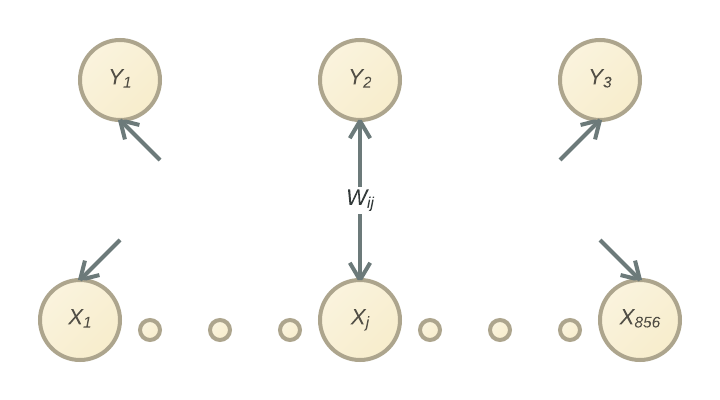
\includegraphics[width=0.7\linewidth]{img/parte1-modelo.png}

	\caption{Modelo de red}
\end{figure}

\subsection{Implementación}

\subsubsection{Prepocesamiento de datos}

El dataset se preprocesa centrando los datos en el 0, calculando la media de las frecuencias de cada palabra (posición del vector) y restándosela a cada una de ellas. De esta forma, la media de cada columna del dataset resultante es 0 y los datos quedan distribuidos alrededor del 0. En este caso, los datos no se normalizan ya que quedarían todas las dimensiones con la misma varianza y la red no podría aprender correctamente.

\subsubsection{Pseudocódigo}

Inicializamos la matriz de pesos con valores random $\in[-1/2, 1/2]$. El dataset se shufflea luego de cargarlo, y se separa en dataset de entrenamiento y de validación.

Elegimos un $lrcons$ igual a 0.07 ya que, luego de realizar varias experimentaciones, observamos que convergía más rápido que otros valores con los que experimentamos.

\begin{algorithm}[H]
\caption{train}
\begin{algorithmic}
	\State e = 0
    \While {not fin}
        \State e+=1
        \State lr = lrcons * e$^{-1}$
        \For {x in dataset}
            \State y = x $\bullet$ weights
            \State aplicamos regla
            \State weights += dw
        \EndFor
    \EndWhile
    \State return weights
\end{algorithmic}
\end{algorithm}

Como criterio de parada para saber que convergió el algoritmo utilizamos que los vectores de la matriz de pesos formen una base ortonormal. 

Para evitar que cicle infinitamente si la matriz de pesos no tiende a una base ortonormal para el $\varepsilon$ que hayamos elegido, optamos por parar el algoritmo si se llega a un máximo de épocas definido.

\begin{algorithm}[H]
\caption{fin}
\begin{algorithmic}
	\State return (e == max\_epochs) or (weights es ortogonal)
\end{algorithmic}
\end{algorithm}

Sabemos que si una matriz $M$ es ortonormal, entonces $M^t \bullet M = I$ donde $I$ es la matriz identidad. Más específicamente, como se trata de valores reales, chequeamos que cada valor de $|M^t \bullet M - I|$ sea menor a $ \varepsilon $ donde $0 < \varepsilon < 0.5$.

\begin{algorithm}[H]
\caption{ortogonal}
\begin{algorithmic}
	\State return ($|$ weigths$^t$ $\bullet$ weights - I $|$ $<$ $\varepsilon$ ).all()
\end{algorithmic}
\end{algorithm}

\subsection{Ejecución}

\subsubsection{Modo de uso}

\textbf{Para entrenar la red:}

\begin{lstlisting}[style=bash]
usage: hbtrain.py [-h] -p P -x X [-n N]

Parametros de la red

optional arguments:
  -h, --help  show this help message and exit
  -p P        Ruta del archivo de salida para guardar la red
  -x X        Ruta de dataset de entrenamiento
  -n N        Cantidad maxima de epochs
\end{lstlisting}

Ejemplo: 

\noindent\texttt{python hbtrain.py -p net.o -x ds/tp2\_training\_dataset.csv -n 100} \\

\textbf{Para cargar datos de validación y visualizar contra los de entrenamiento:}

\begin{lstlisting}[style=bash]
usage: hbreduction.py [-h] -p P -x X

Parametros de la red

optional arguments:
  -h, --help  show this help message and exit
  -p P        Ruta del archivo de entrada con la red
  -x X        Ruta de dataset de validacion
\end{lstlisting}

Ejemplo:

\noindent\texttt{python hbreduction.py -p net.o -x ds/tp2\_testing\_dataset.csv} \\

\subsubsection{Requerimientos}

Python:
\begin{itemize}
\item Numpy 
\item Matplotlib
\end{itemize}

\subsection{Resultados}

A continuación, se pueden observar representaciones gráficas de las posiciones en el espacio $\mathbb{R}^3$ que el modelo le asigna a cada documento, con la red entrenada con 600 datos y 300 datos de validación.

\subsubsection{Oja}

\begin{figure}[ht!]
	\centering
	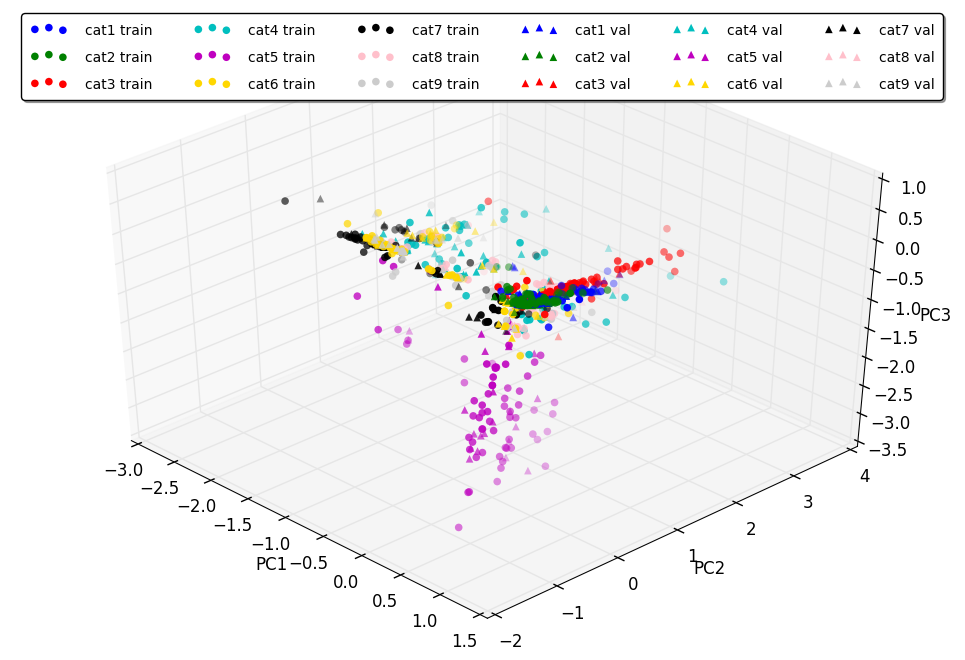
\includegraphics[width=0.9\linewidth]{img/parte1-vista3d-oja.png}

	\caption{Vista 3d de datos reducidos a tres dimensiones con regla Oja}
\end{figure}

\begin{figure}[ht!]	
	\begin{subfigure}[b]{0.5\textwidth}
		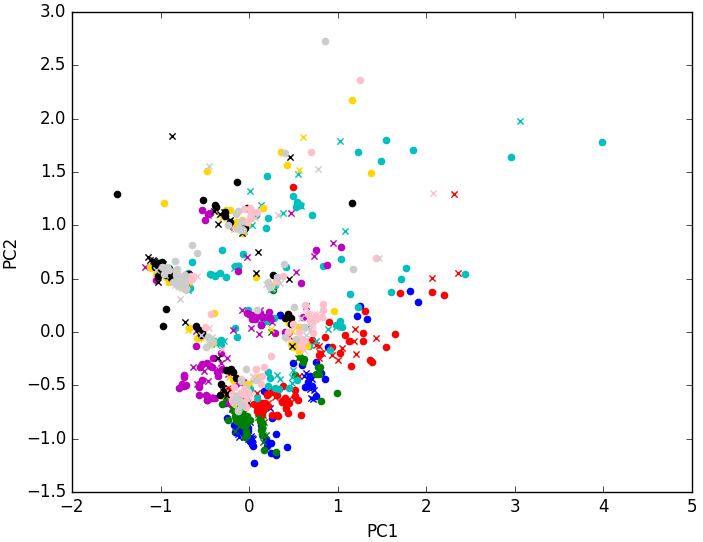
\includegraphics[width=\linewidth]{img/oja/3dim-pc1-pc2.png}
	\end{subfigure}%
	~
	\begin{subfigure}[b]{0.5\textwidth}
		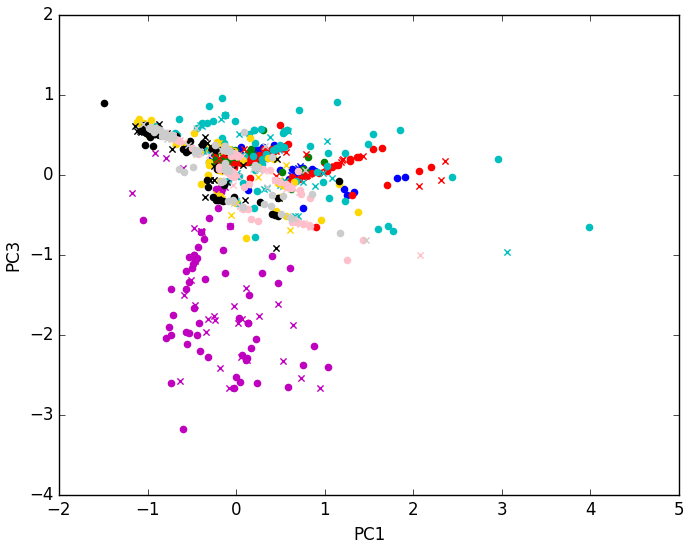
\includegraphics[width=\linewidth]{img/oja/3dim-pc1-pc3.png}
	\end{subfigure}%

\end{figure}


\begin{figure}[ht!]	
	~\centering
	\begin{subfigure}[b]{0.5\textwidth}
		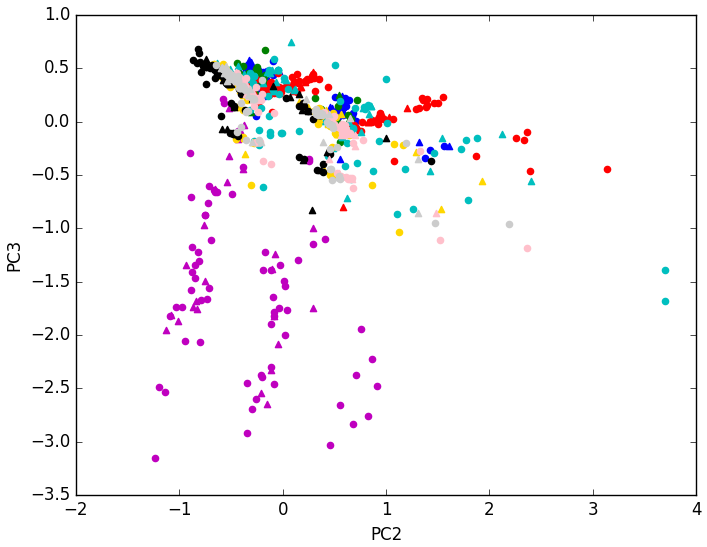
\includegraphics[width=\linewidth]{img/oja/3dim-pc2-pc3.png}
	\end{subfigure}%
	\caption{Vistas de dos dimensiones}
\end{figure}


\subsubsection{Sanger}

\begin{figure}[ht!]
	\centering
	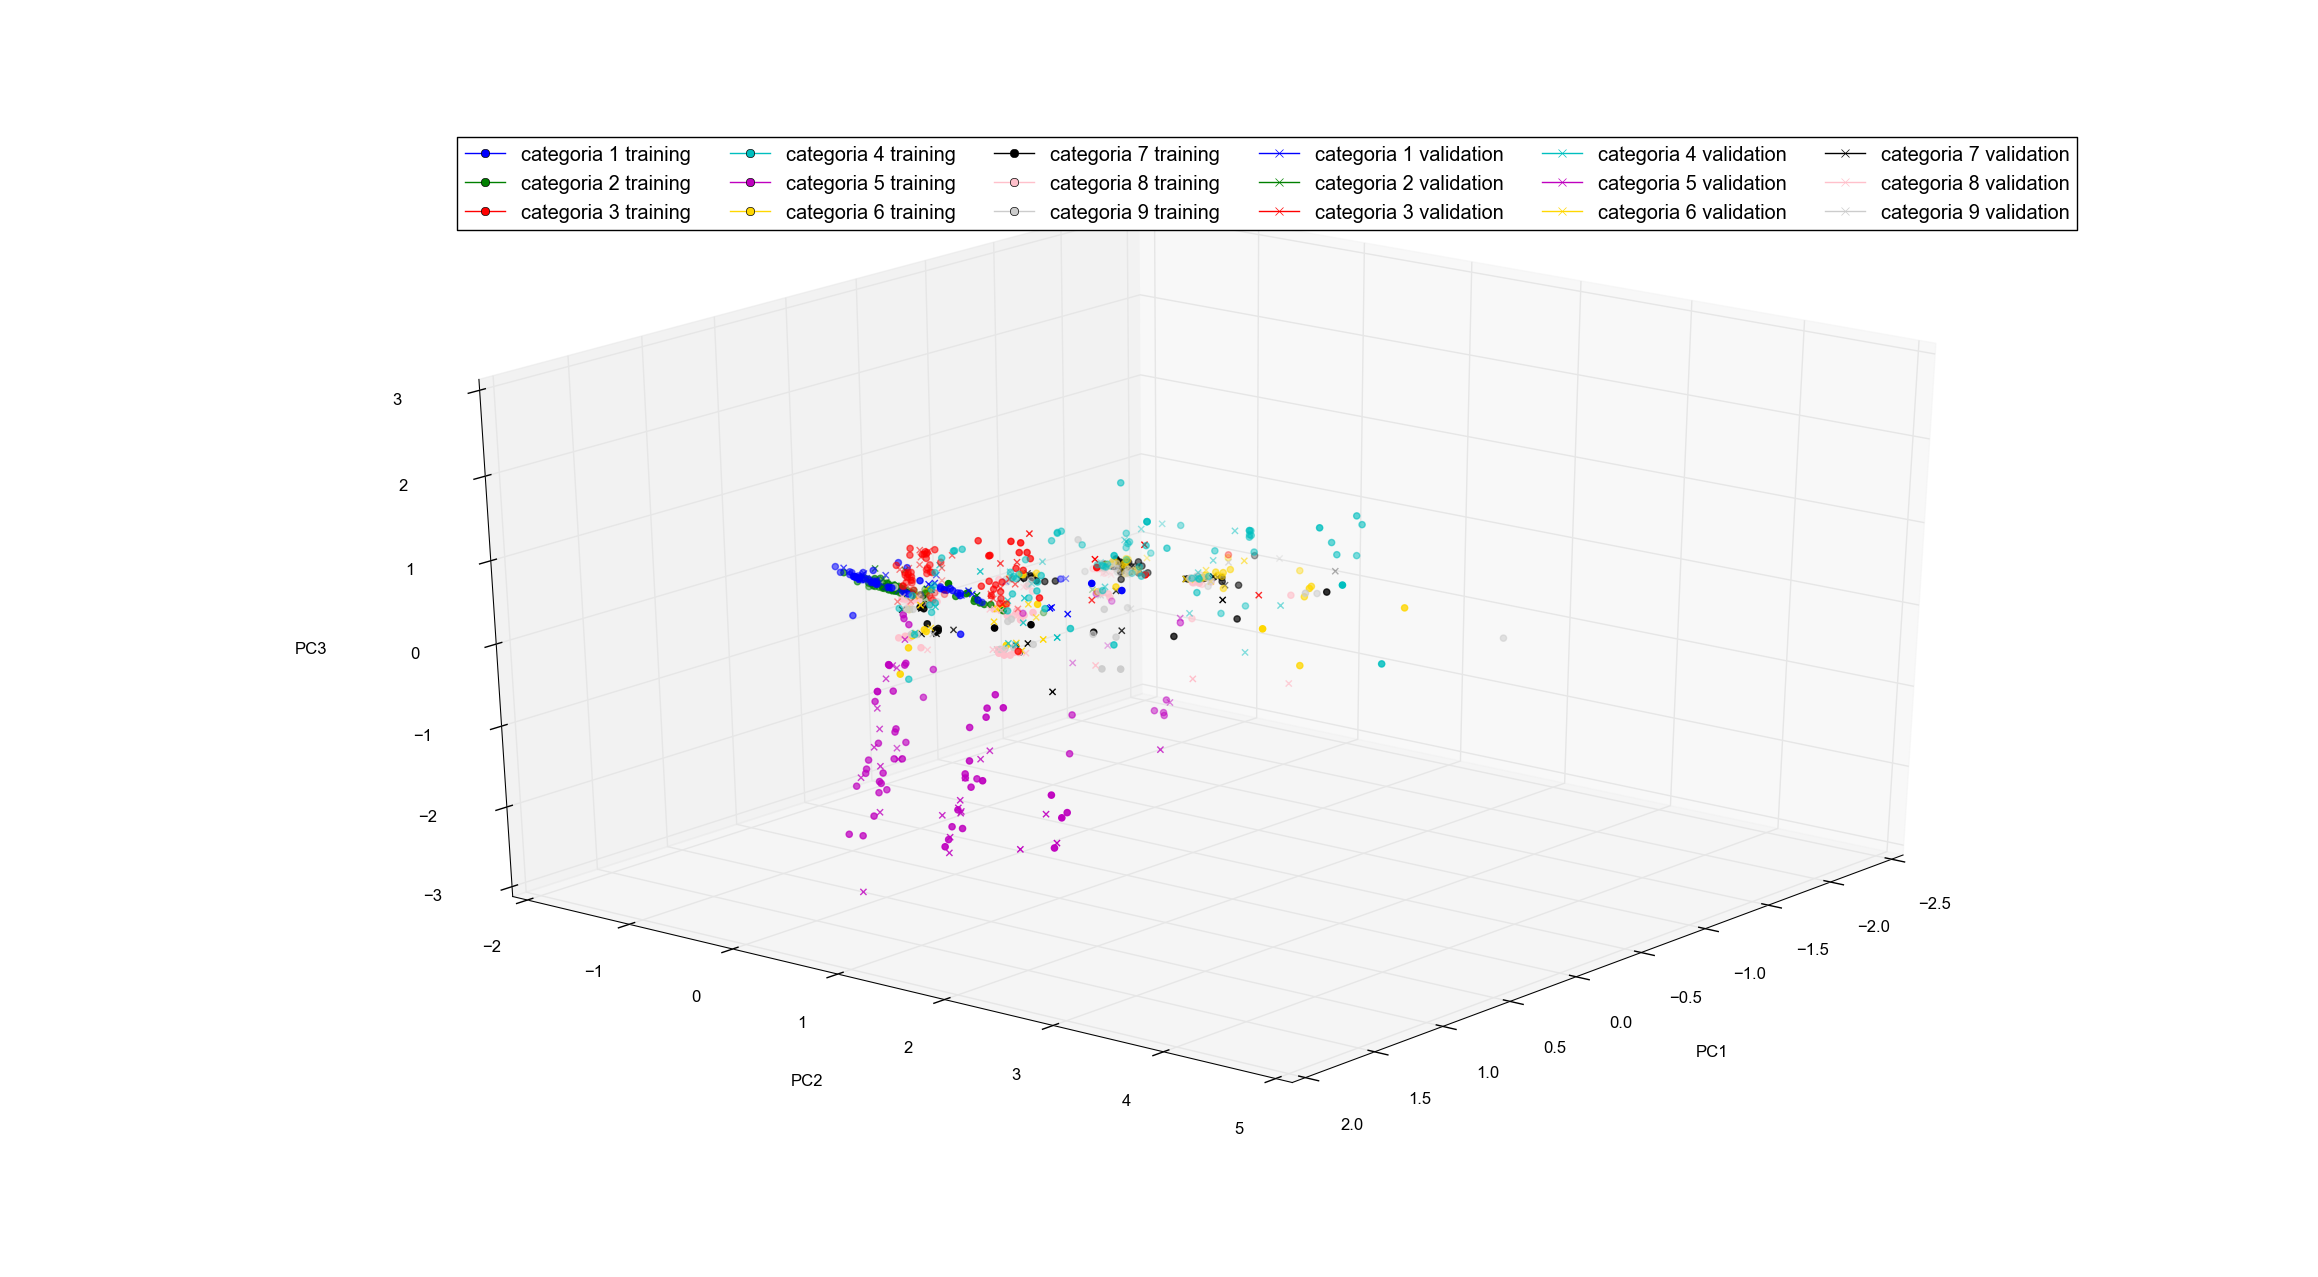
\includegraphics[width=0.9\linewidth]{img/parte1-vista3d-sanger.png}

	\caption{Vista 3d de datos reducidos a tres dimensiones con regla Sanger}
\end{figure}

\begin{figure}[ht!]	
	\begin{subfigure}[b]{0.5\textwidth}
		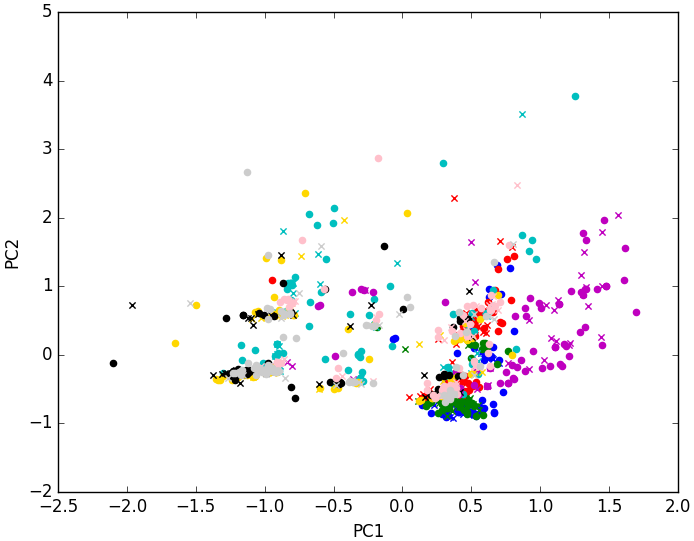
\includegraphics[width=\linewidth]{img/sanger/3dim-pc1-pc2.png}
	\end{subfigure}%
	~
	\begin{subfigure}[b]{0.5\textwidth}
		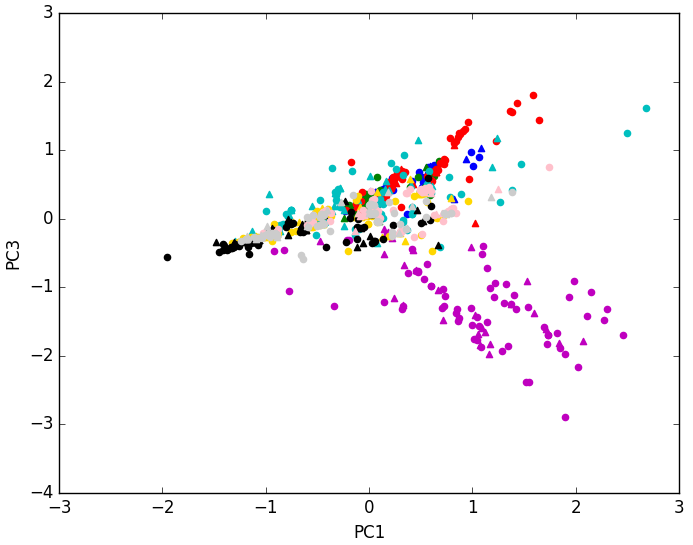
\includegraphics[width=\linewidth]{img/sanger/3dim-pc1-pc3.png}
	\end{subfigure}%

\end{figure}

\begin{figure}[ht!]	
	~\centering
	\begin{subfigure}[b]{0.5\textwidth}
		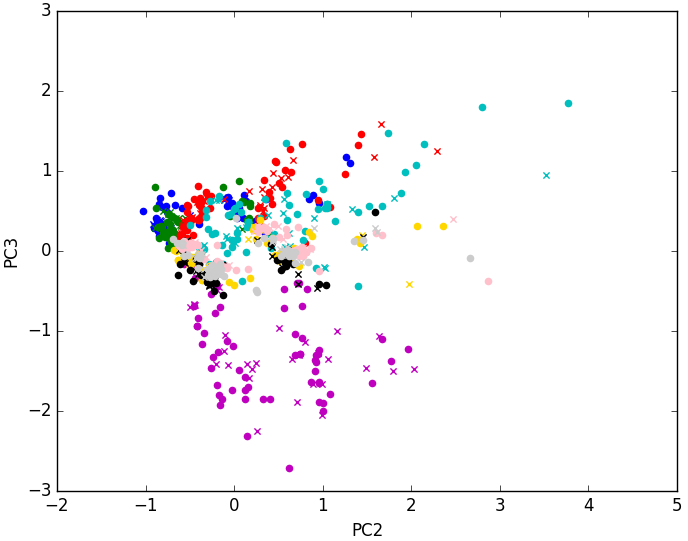
\includegraphics[width=\linewidth]{img/sanger/3dim-pc2-pc3.png}
	\end{subfigure}%
	\caption{Vistas de dos dimensiones}
\end{figure}



\subsection{Conslusiones}

Observando las representaciones gráficas en la sección de resultados de los datos reducidos obtenidos con el modelo de red propuesto de 3 unidades de salida, podemos concluir que este modelo de red no resulta bueno para la clasificación de estos documentos. Los datos reducidos de las distintas categorías no se diferencian bien. Esto se debe a que reducimos a sólo 3 dimensiones, tenemos 9 categorías y, además, que el número de categoría de cada documento corresponde a la actividad principal de la empresa, no necesariamente la única. 

Para obtener mejores resultados, proponemos un modelo de red con 9 unidades de salida. Si bien esto complica la visualización de los datos reducidos, ya que tendríamos 9 dimensiones, se puede hacer una representación gráfica en dos dimensiones de cada par de componentes principales y analizar los datos en conjunto.



